\documentclass[a4paper, 12pt]{article}

\usepackage[T2A]{fontenc}
\usepackage[utf8]{inputenc}
\usepackage[english, russian]{babel}
\usepackage{amsmath}
\usepackage{graphicx}
\usepackage{subcaption}
\usepackage{float}
\usepackage{tabularx}
\usepackage{amsmath,booktabs}
\usepackage{array}
\righthyphenmin=2
\usepackage[left=20mm, top=20mm, right=20mm, bottom=20mm]{geometry} % настройки полей документа
\usepackage{caption}
\usepackage{makecell}

% Paragraph indent
\usepackage{indentfirst}
\setlength{\parindent}{15mm}

%%%%%%%TITUL%%%%%%%
\newcommand\tline[2]{$\underset{\text{#1}}{\text{\underline{\hspace{#2}}}}$}

%%%%%%%%%%%%CAPTION%%%%%%%
\usepackage{threeparttable}
%Change label separator
\usepackage{caption}
\captionsetup[table]{labelformat=simple, labelsep = endash, justification = raggedright, singlelinecheck = off, width = 0.75\textwidth}
\captionsetup[figure]{labelformat=simple, labelsep = endash, name = Рисунок}
%%%%%%%TABLE%%%%
\renewcommand{\arraystretch}{1.3}
\renewcommand{\tabcolsep}{0.5cm}

%%%%%%%%%%%%%%%%%%%%%%%%%%%%%%%%%%
\begin{document} 
	
		\begin{titlepage}
		\centering
		{\fontsize{12pt}{5cm}\selectfont \bfseries Министерство образования и науки Российской Федерации} \\ \vspace{0.5cm}
		{\fontsize{7pt}{5cm}\selectfont ФЕДЕРАЛЬНОЕ ГОСУДАРСТВЕННОЕ АВТОНОМНОЕ ОБРАЗОВАТЕЛЬНОЕ УЧРЕЖДЕНИЕ ВЫСШЕГО ПРОФЕССИОНАЛЬНОГО ОБРАЗОВАНИЯ} \\ 
		\vspace{1cm}
		{\fontsize{12pt}{5cm}\selectfont \bfseries САНКТ-ПЕТЕРБУРГСКИЙ УНИВЕРСИТЕТ ИНФОРМАЦИОННЫХ ТЕХНОЛОГИЙ, МЕХАНИКИ И ОПТИКИ} \\ \vspace{1.5cm}
		
		{\fontsize{14pt}{5cm}\selectfont Кафедра \hspace{1cm} \underline{Систем Управления и Информатики}  \hspace{1cm} Группа \underline{Р3340}} \\ 
		\vspace{2cm}
		
		{\fontsize{20pt}{5cm}\selectfont \bfseries Лабораторная работа №10} \\
		{\fontsize{20pt}{5cm}\selectfont \bfseries “Исследование математической модели электромеханического объекта управления”} \\
		{\fontsize{14pt}{5cm}\selectfont Вариант - 02} \\
		\vspace{1.5cm}
		
		\flushleft
		
		{Выполнил \hspace{0.5cm} \tline{(фамилия, и.о.)}{10cm} (подпись)} \\
		\vspace{2cm}
		
		{Проверил \hspace{0.5cm} \tline{(фамилия, и.о.)}{10cm} (подпись)} \\
		\vspace{5cm}
		
		"\underline{\hspace{0.4cm}}"\hspace{0.1cm}\underline{\hspace{1.5cm}}\hspace{0.1cm}20\underline{\hspace{0.4cm}}г. \hspace{2cm} Санкт-Петербург, \hspace{2cm} 20\underline{\hspace{0.4cm}}г. \\ \vspace{1cm}
		
		Работа выполнена с оценкой \hspace{0.5cm} \underline{\hspace{10cm}} \\ 
		\vspace{1cm}
		Дата защиты "\underline{\hspace{0.4cm}}"\hspace{0.1cm}\underline{\hspace{1.5cm}}\hspace{0.1cm}20\underline{\hspace{0.4cm}}г.
		
		\end{titlepage}


\section*{Цель работы}
	Изучение математических моделей и исследование характеристик электромеханического объекта управления, построенного на основе электродвигателя постоянного тока независимого возбуждения.
\section*{Исходные данные}
Функциональная схема исследуемого электромеханического объекта и исходные данные к нему представлены на рисунке \ref{EMO} и таблице \ref{tab:dateTab}
	\begin{figure}[h!]
		\centering
		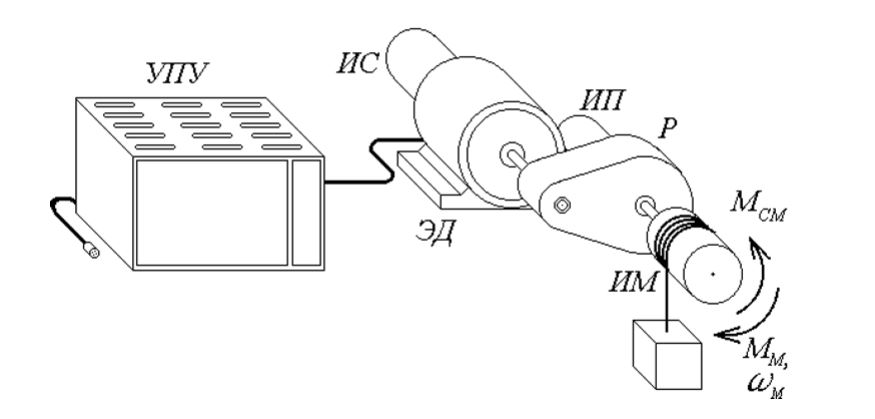
\includegraphics[width = 1\textwidth]{EMO}
		\caption{Функциональная схема ЭМО}
		\label{EMO}
	\end{figure}

\begin{table}[h!]
	\centering
	\begin{threeparttable}
		\caption{Исходные данные}
		\begin{tabular}{|c|c|c|c|c|c|c|c|c|c|}
			\hline
			\makecell{$U_\text{Н},$\\В} & \makecell{$n_0,$\\об/мин} & \makecell{$I_\text{Н},$\\A} & \makecell{$M_\text{Н},$\\Н$\cdot$м} & \makecell{R,\\Ом} & \makecell{$T_\text{Я},$\\мс} & \makecell{$J_\text{Д},$\\кг$\cdot$м$^2$} & \makecell{$T_\text{У},$\\мс} &
			$i_\text{Р}$
			& \makecell{$J_\text{М},$\\кг$\cdot$м$^2$} \\
			\hline
			48 & 1000 & 12 & 5,5 & 0,75 & 5 & $1,6\cdot10^{-3}$ & 6 & 16 & 2,75\\
			\hline
		\end{tabular}
		\label{tab:dateTab}
	\end{threeparttable}
\end{table}

\newpage

\begin{center}
	\section{Расчет параметров математической модели двигателя}
\end{center}\par
Рассчитаем по исходным данным дополнительные параметры моделирования.\par

\begin{gather}
	K_y  = \frac{U_\text{Н}}{U_m}  = 4.8\\
	w_0  = n_0\frac{\pi}{30} = 104.72 \\
	K_e  = \frac{U_\text{Н}}{w_0} = 0.4584\\
	K_\text{Д}  = \frac{1}{R} = 1.33 \\
	K_\text{М}  = \frac{M_\text{Н}}{I_\text{Н}} =  0.4583\\
	J_{\Sigma}  = 1.2J_\text{Д} + \frac{J_\text{М}}{i^2_p} = 0.0127
\end{gather} \par
Коэффициенты передачи измерительных устройств $K_U, K_I, K_\omega, K_\alpha$ выбираются таким образом, чтобы обеспечить соответствие максимального значения измеряемого сигнала уровню 10 В на выходе измерительного устройства. В итоге получим следующие значения коэффициентов:
\begin{gather}
	K_U = \frac{\hat{U}_{ymax}}{U_\text{Н}} = \frac{10}{24} = 0.4167\\
	K_I = \frac{\hat{I}_{max}}{I_{max}} = \frac{10}{34.18} =  0.4168\\
	K_\omega = \frac{\hat{\omega}_{max}}{\omega_0} = \frac{10}{52.36} = 0.1910\\
	K_\alpha = \frac{\hat{\alpha}_{max}}{\alpha_{max}} = \frac{10}{32.55} = 0.3071
\end{gather}

\newpage

\begin{center}
	\section{Вывод моделей ВСВ для полной схемы моделирование ЭМО}
\end{center} \par

Запишем уравнения, описывающие работу ЭМО. 
\begin{equation}
\begin{cases}
k_\text{м}I - M_c = J_\Sigma \dot{\omega} \\
T_\text{я}\dot{I} + I = k_\text{д}U_y - k_\text{д}k_e\omega \\
T_y\dot{U_y} + U_y = k_yU
\end{cases} \Leftrightarrow
\begin{cases}
\dot{\omega} = \frac{k_\text{м}}{J_\Sigma}I - \frac{1}{J_\Sigma}M_c \\
\dot{I} = - \frac{k_\text{д}k_e}{T_\text{я}}\omega - \frac{1}{T_\text{я}}I + \frac{k_\text{д}}{T_\text{я}}U_y \\
\dot{U_y} = -\frac{1}{T_y}U_y + \frac{k_y}{T_y}U
\end{cases}
\end{equation} \par
Примем вектор состояния $X = \begin{bmatrix} \alpha & \omega & I & U_y \end{bmatrix}^T$ и $\dot{\alpha} = \omega$, получим следующую модель вход состояние выход (ВСВ)

	\begin{align}
		\begin{bmatrix}
			\dot{\alpha} \\
			\dot{\omega} \\
			\dot{I} \\
			\dot{U_y} 
		\end{bmatrix} & = 
		\begin{bmatrix}
			0 & 1 & 0 & 0 \\
			0 & 0 & \frac{k_\text{м}}{J_\Sigma} & 0 \\
			0 & -\frac{k_\text{д}k_e}{T_\text{я}} & - \frac{1}{T_\text{я}} & \frac{k_\text{д}}{T_\text{я}} \\
			0 & 0 & 0 & -\frac{1}{T_y}
		\end{bmatrix}
		\begin{bmatrix}
			\alpha \\
			\omega \\
			I \\
			U_y 
		\end{bmatrix} + 
		\begin{bmatrix}
			0 & 0 \\
			0 & - \frac{1}{J_\Sigma} \\
			0 & 0 \\
			\frac{k_y}{T_y} & 0
		\end{bmatrix}
		\begin{bmatrix}
			U(t) \\
			M_c(t)
		\end{bmatrix} \\
		\alpha & = 
		\begin{bmatrix}
			1 & 0 & 0 & 0
		\end{bmatrix}
		\begin{bmatrix}
			\alpha \\
			\omega \\
			I \\
			U_y 
		\end{bmatrix}
	\end{align}
	
\newpage

\begin{center}
	\section{Моделирование электромеханического объекта}
\end{center}
На рисунке \ref{strEMO} представлена структурная схема моделирования электромеханического объекта, а на рисунке \ref{funcEMO}  - функциональная.

\begin{figure}[h!]
	\centering
	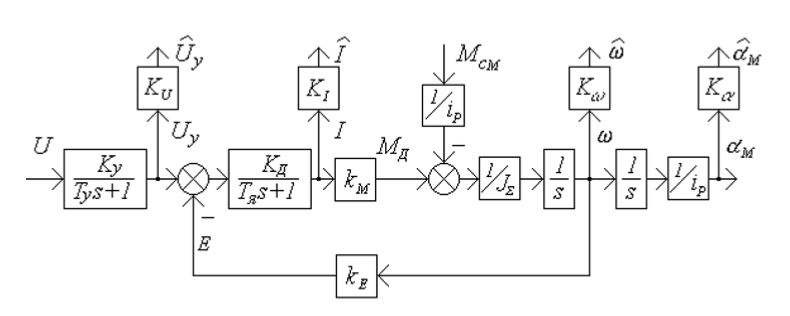
\includegraphics[width = 1\textwidth]{strEMO}
	\caption{Структурная схема схема ЭМО}
	\label{strEMO}
\end{figure}
\begin{figure}[h!]
	\centering
	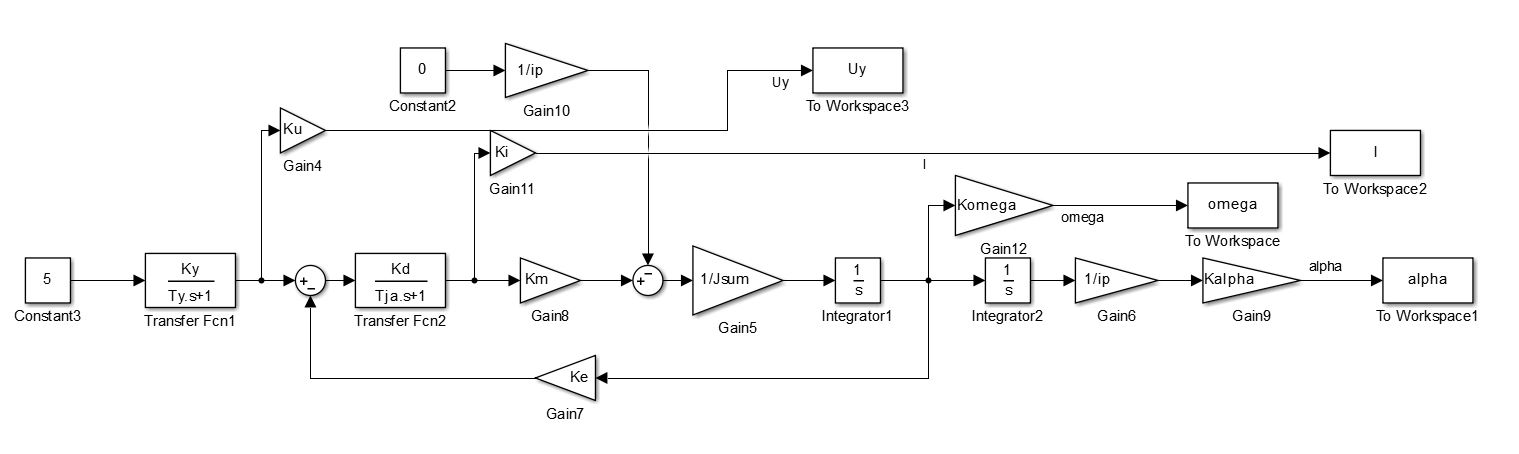
\includegraphics[width = 1\textwidth]{fullmod}
	\caption{Функциональная схема схема ЭМО}
	\label{funcEMO}
\end{figure}

Рассмотрим переходные процессы полной модели ЭМО.
На рисунке \ref{begin} изображены графики напряжения $U_y$, тока $I$, скорости $\omega$ и угла $\alpha$.

\newpage
\begin{figure}[h!]
	\centering
	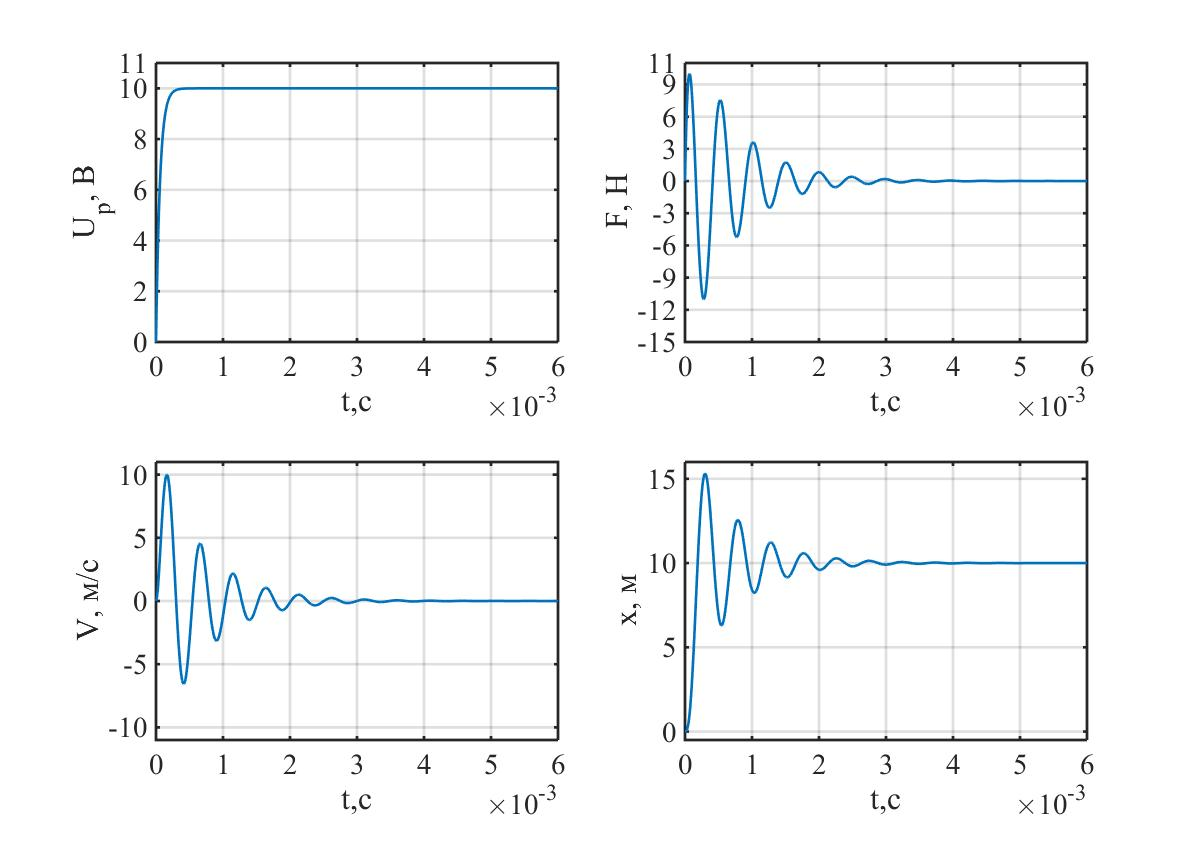
\includegraphics[width = 1\textwidth]{data/begin}
	\caption{Графики переходных процессов при $M_{cm}=0$ Нм и $U=5$ В}
	\label{begin}
\end{figure}  

\newpage
\begin{center}
\section{Исследование влияния момента сопротивления на вид переходных процессов}
\end{center}\par
Для исследования влияния момента сопротивления на ЭМО необходимо изменять момент сопротивления $M_{cm}=0$ от 0 до $i_p*M_n=88$. Полученные графики приведены на рисунке \ref{moment}

\begin{figure}[h!]
	\centering
	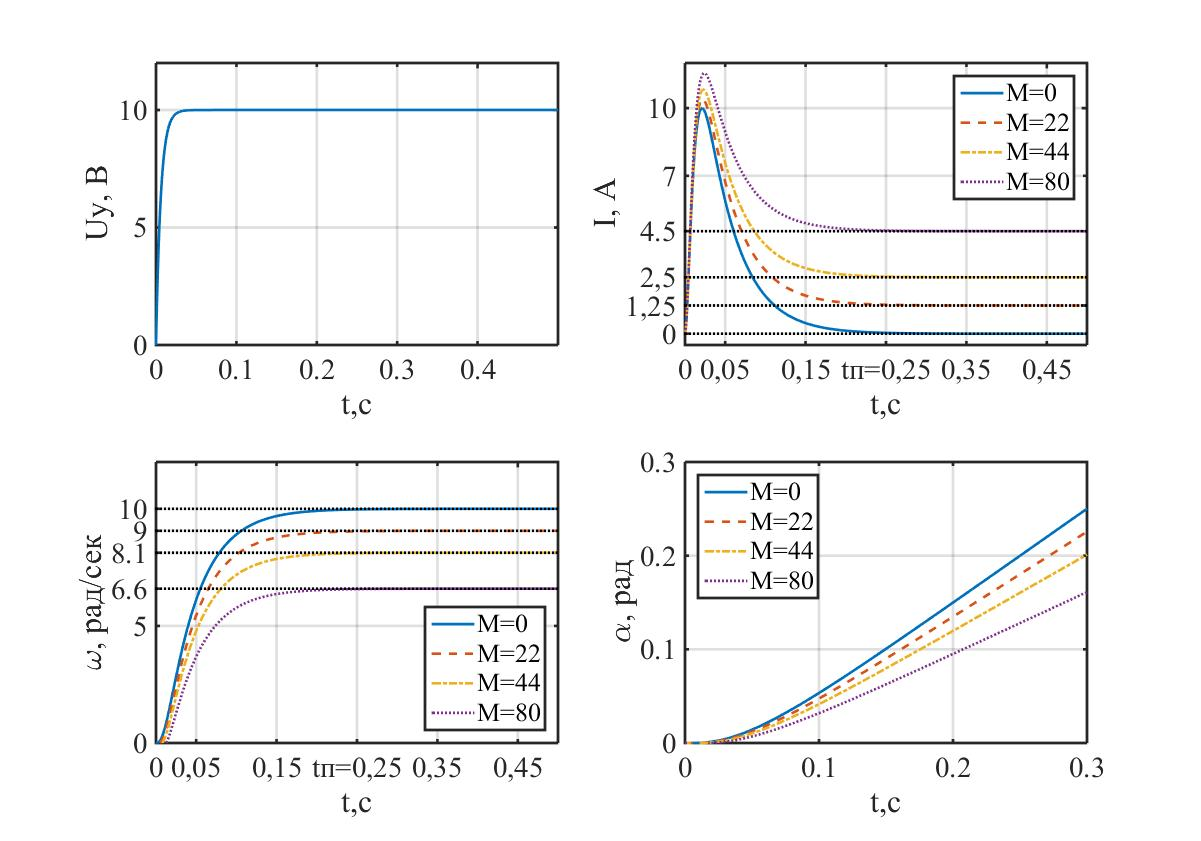
\includegraphics[width = 1\textwidth]{data/moment}
	\caption{Графики переходных процессов при изменении момента}
	\label{moment}
\end{figure}  
В ходе эксперимента, изменяя нагрузочный момент, мы получили различные значения времени, установившиеся значения тока, угловой скорости переходного процесса, которые представлены в таблице \ref{tab:moment}.

\begin{table}[h!]
	\centering
	\begin{threeparttable}
		\caption{Установившихся значения при $M_{cm}$}
		\begin{tabular}{|c|c|c|c|}
			\hline
			$M_{cm}$, Нм	&	$t_\text{п}$, с	&	$\omega_y$, рад/сек	&	$I_y$, А\\
			\hline
			0		&	0.25			&	10			&	0\\
			\hline
			22		&	0.25			&	9			&	1.25\\
			\hline
			44		&	0.25			&	8.1			&	2.5\\
			\hline
			80		&	0.25			&	6.6			&	4.5\\
			\hline
			
		\end{tabular}
		\label{tab:moment}
	\end{threeparttable}
\end{table}

\newpage
\begin{center}
\section{Исследование влияния момента инерции нагрузки $J_\text{М}$}
\end{center}
На рисунке \ref{Jm} представлены графики переходных процессов при различных значениях момента инерции нагрузки $J_\text{М}$.

\begin{figure}[h!]
	\centering
	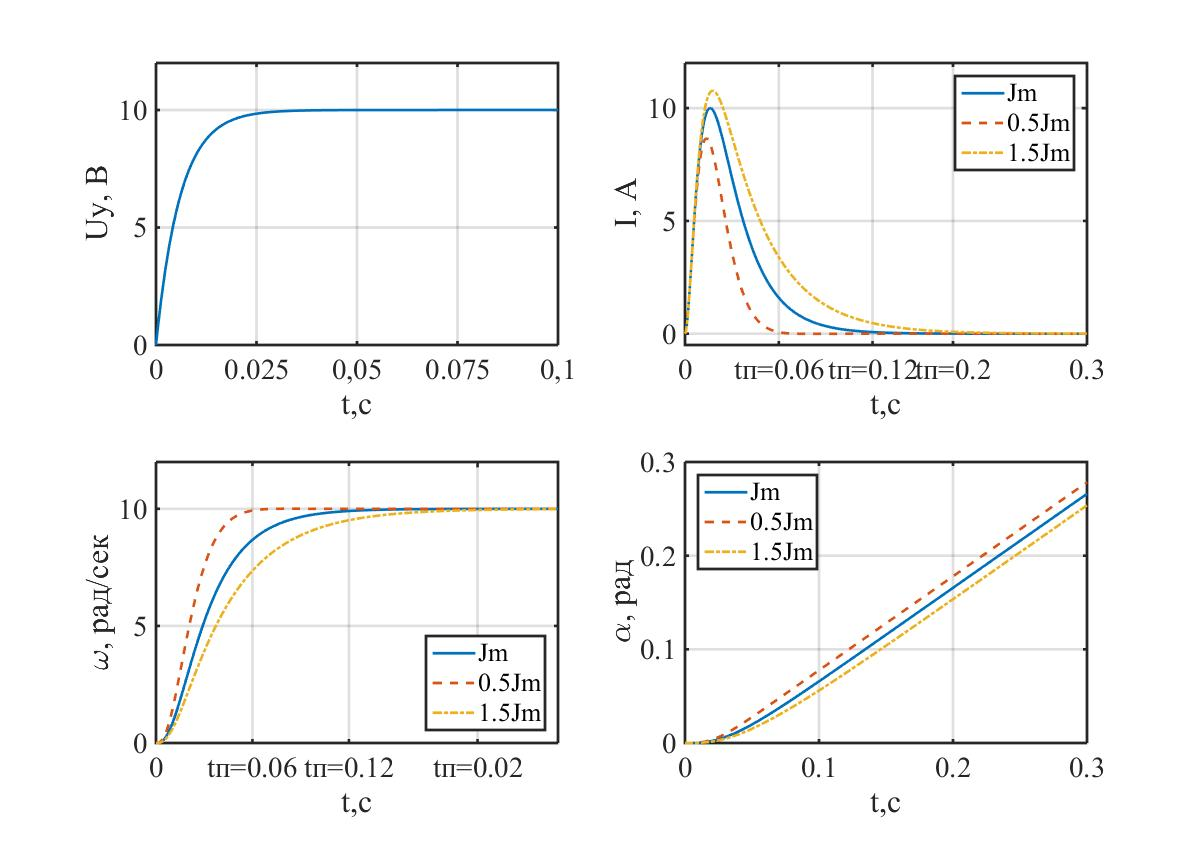
\includegraphics[width = 1\textwidth]{data/Jm}
	\caption{Графики переходных процессов при различных $J_\text{М}$}
	\label{Jm}
\end{figure}

В ходе эксперимента, изменяя момент инерции нагрузки, мы получили различные значения времени, установившиеся значения тока, угловой скорости переходного процесса, которые представлены в таблице \ref{tab:Jm}.

\begin{table}[h!]
	\centering
	\begin{threeparttable}
		\caption{Установившихся значения при $J_\text{М}$}
		\begin{tabular}{|c|c|c|c|}
			\hline
			$J_\text{М}$, Нм	&	$t_\text{п}$, с	&	$\omega_y$, рад/сек	&	$I_y$, А\\
			\hline
			$1.37=0.5J_\text{М}$		&	0.12	&	10		&	0\\
			\hline
			$2.75=J_\text{М}$		&	0.25	&	10		&	0\\
			\hline
			$4.12=1.5J_\text{М}$		&	0.35		&	10		&	0\\
			\hline			
		\end{tabular}
		\label{tab:Jm}
	\end{threeparttable}
\end{table}

\newpage
\begin{center}
	\section{Исследование влияния передаточного отношения $i_p$}
\end{center}\par
На рисунках \ref{ipm0} и представлены графики преходных процессов при различных значениях передаточного отношения и нулевом моменте нагрузки $M_\text{СМ} = 0$ и при $M_\text{СМ} = 44$.

\begin{figure}[h!]
	\centering
	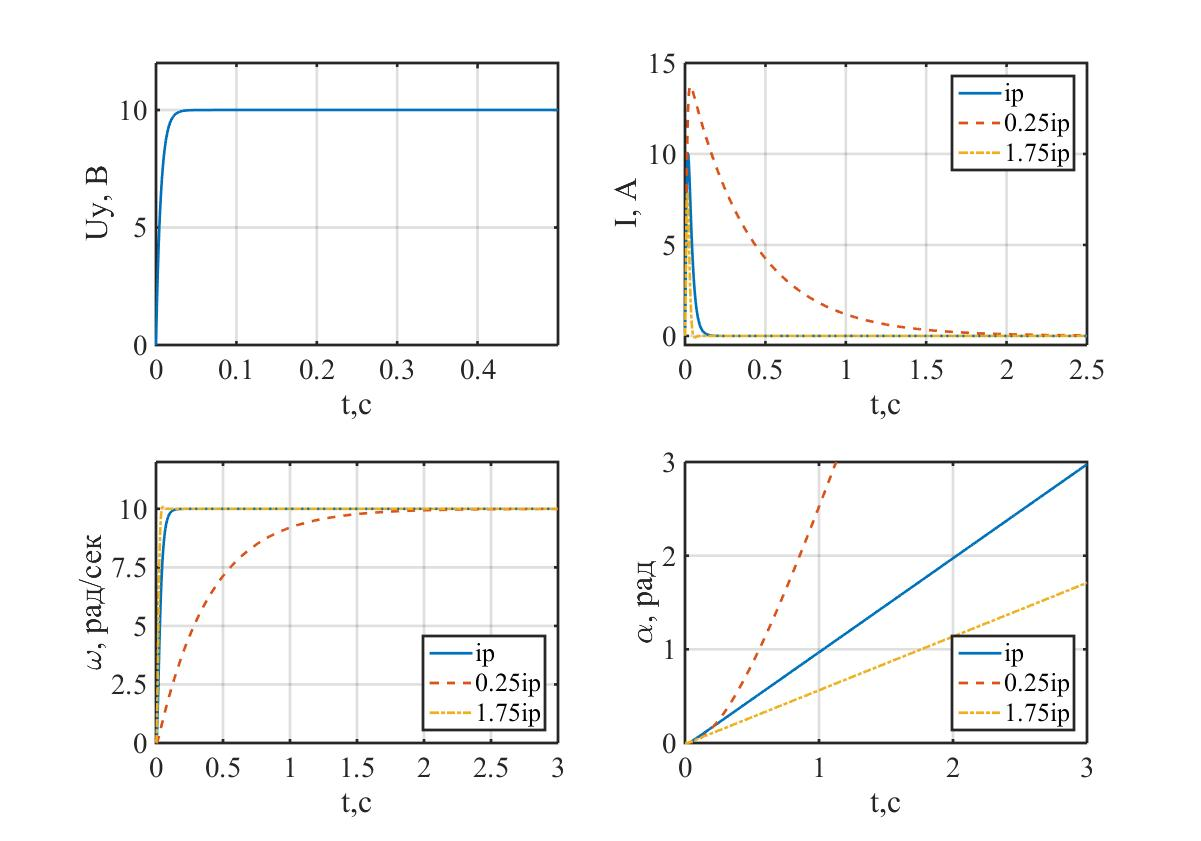
\includegraphics[width = 1\textwidth]{data/ipm0}
	\caption{Графики прехеходных процессов при различных $i_p$ и $M_\text{СМ} = 0$ Нм}
	\label{ipm0}
\end{figure}
\newpage
\begin{figure}[h!]
	\centering
	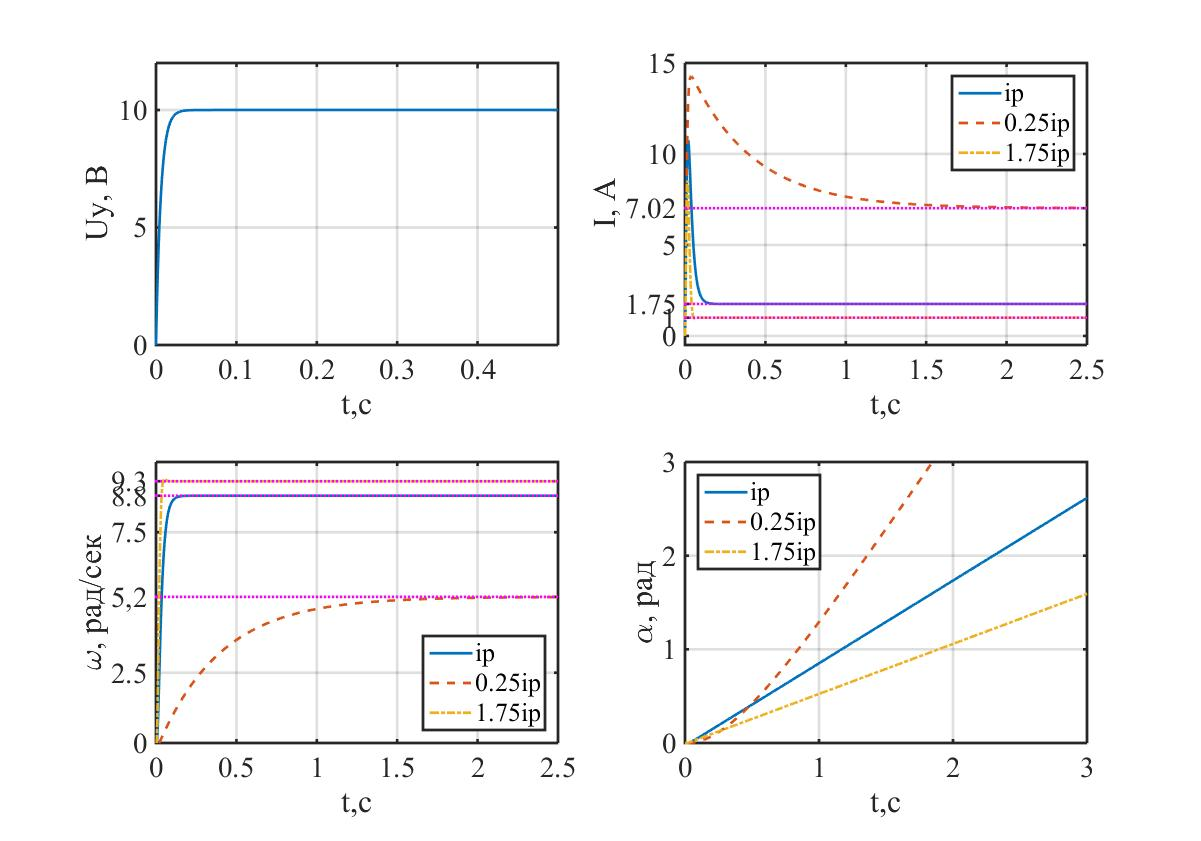
\includegraphics[width = 1\textwidth]{data/ipm44}
	\caption{Графики прехеходных процессов при различных $i_p$ и $M_\text{СМ} = 44$ Нм}
	\label{ipm44}
\end{figure}
\newpage
\section{Вывод модели ВСВ для упрощенной схемы моделирования ЭМО}
Для составления упрощенной модели ЭМО приравниваем постоянные времени $T_\text{я}$ и $T_y$ к 0, так как их значения существенно меньше $T_m$. Получим следующие выражения:

\begin{equation}
\begin{cases}
\dot{\alpha} = \omega \\
\dot{\omega} = -\frac{k_\text{м}k_\text{д}k_e}{J_\Sigma}\omega + \frac{k_\text{м}k_\text{д}k_y}{J_\Sigma}U - \frac{1}{J_\Sigma}M_c
\end{cases}
\end{equation}

Исходя из данной системы можно построить модель ВСВ.
\begin{align}
\begin{bmatrix}
\dot{\alpha} \\
\dot{\omega} \\
\end{bmatrix} & = 
\begin{bmatrix}
0 & 1 \\
0 & -\frac{k_\text{м}k_\text{д}k_e}{J_\Sigma} \\
\end{bmatrix}
\begin{bmatrix}
\alpha \\
\omega \\
\end{bmatrix} + 
\begin{bmatrix}
0 & 0 \\
\frac{k_\text{м}k_\text{д}k_y}{J_\Sigma} & -\frac{1}{J_\Sigma} \\
\end{bmatrix}
\begin{bmatrix}
U(t) \\
M_c(t)
\end{bmatrix} \\
\alpha & = 
\begin{bmatrix}
1 & 0 
\end{bmatrix}
\begin{bmatrix}
\alpha \\
\omega \\
\end{bmatrix}
\end{align}

\newpage
\begin{center}
	\section{Моделирование упрощенной моделей ЭМО}
\end{center}\par
На рисунке \ref{nstrEMO} представлена структурная схема упрощенной модели ЭМО, а на рисунке \ref{nfuncEMO}  - функциональная.

\begin{figure}[h!]
	\centering
	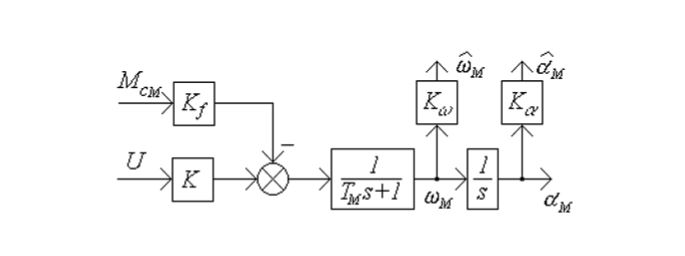
\includegraphics[width = 1\textwidth]{notfullstrEMO}
	\caption{Структурная схема упрощенной модели ЭМО}
	\label{nstrEMO}
\end{figure}

\begin{figure}[h!]
	\centering
	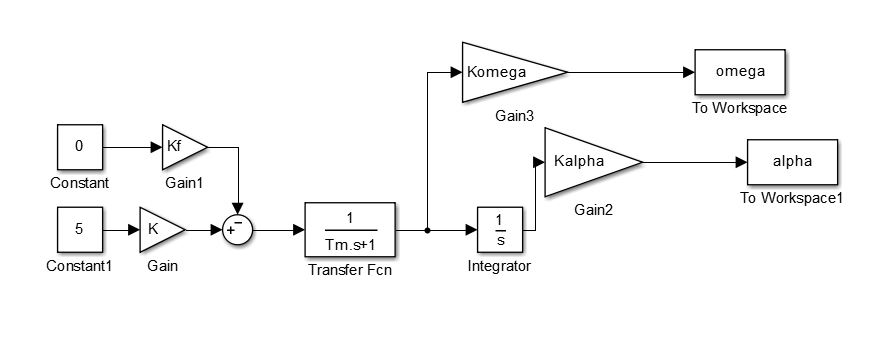
\includegraphics[width = 1\textwidth]{notfullmod}
	\caption{Структурная схема упрощенной модели ЭМО}
	\label{nfuncEMO}
\end{figure}
Сравним переходные характеристики полной и упрощенной модели на рисунке \ref{full_nfull}
\newpage
\begin{figure}[h!]
	\centering
	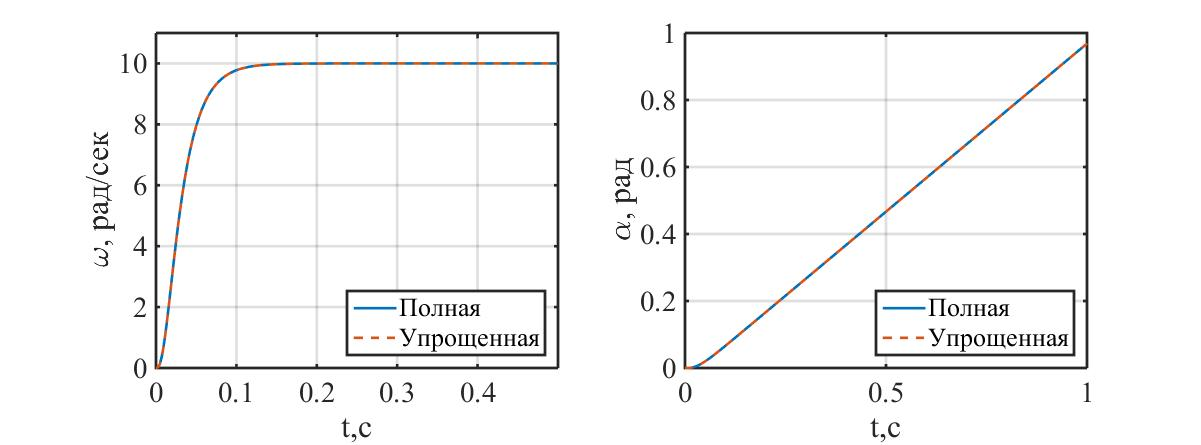
\includegraphics[width = 1\textwidth]{data/full_notfull}
	\caption{Структурная схема упрощенной модели ЭМО}
	\label{full_nfull}
\end{figure}
 
\newpage

\begin{center}
	\section*{Вывод}
\end{center}\par
В ходе работы было исследовано различное влияние моментов нагрузки, инерции, передаточных моментов редуктора и постоянных времени на модель электромеханического объекта.\par
Было выявлено, что, при увеличении момента инерции, увеличивается время переходных процессов, при увеличении момента сопротивления , увеличивается установившееся значение тока якоря и уменьшается установившееся значение угловой скорости, а изменение передаточного момента редуктора влияет только при наличии нагрузочного момента.\par
Так же была исследована упрощенная модель ЭМО, которая подтверждает, что при достаточно малых постоянных времени у электрических процессов по сравнению с механическими можно использовать упрощенную модель ЭМО.




\end{document} 